
\documentclass[english,12pt,a4paper,pdftex]{article}
%% This package is required
%% Choose your school from arts, biz, chem, elec, eng, sci.
%% Choose the character encoding scheme used by your editor: utf8, latin1

\usepackage[elec,utf8]{aaltothesis} % this is the default in aaltothesis.sty
%% Use this if you run pdflatex and use jpg/pdf-format pictures.

\usepackage{graphicx}

%% Use the macros in this package to change how the hyperref package below 
%% typesets its hypertext -- hyperlink colour, font, etc. See the package
%% documentation. It also defines the \url macro, so use the package when 
%% not using the hyperref package.
%\usepackage{url}

%%% For fancy tables (Jose)
\usepackage{multirow}
\usepackage{chngpage}
\usepackage{booktabs}
\usepackage{framed}
\usepackage{longtable}

%% Use this if you want to get links and nice output with pdflatex
\usepackage[pdfpagemode=None,colorlinks=true,urlcolor=red,%
linkcolor=blue,citecolor=black,pdfstartview=FitH]{hyperref}

%% Use this if you write hard core mathematics, these are usually needed
\usepackage{amsfonts,amssymb,amsbsy}  

%% For listing code
\usepackage{xcolor,listings}

%% Horizontal margins, DO NOT TOUCH!
\setlength{\hoffset}{-1in}
\setlength{\oddsidemargin}{35mm}
\setlength{\evensidemargin}{25mm}
\setlength{\textwidth}{15cm}
%% Vertical margins, DO NOT TOUCH!
\setlength{\voffset}{-1in}
\setlength{\headsep}{7mm}
\setlength{\headheight}{1em}
\setlength{\topmargin}{25mm-\headheight-\headsep}
\setlength{\textheight}{23cm}

%% Output starts here
\begin{document}
%% Change the school field to describe your school if the autimatically 
%% set name is wrong
% \university{aalto University}{aalto-Yliopisto}
% \school{School of Electrical Engineering}{SähköTekniikan korkeakoulu}

%% Vain kandityölle: Korjaa seuraavat vastaamaan koulutusohjelmaasi
%%
%% Only for B.Sc. thesis: Choose your degree programme. 
%\degreeprogram{Electronics and electrical engineering}%

%% Only for M.Sc. and Licentiate thesis: Choose your department,
%% professorship and professorship code. 
\department{Department of Signal Processing and Acoustics}%
{Signaalinkäsittelyn ja akustiikan laitos}
\professorship{Speech and Language Processing}{}
\code{S-89}

%% Choose one of these:
%\univdegree{BSc}
%\univdegree{MSc}
%% Added by Jose: For the non-finnish/swedish, the Lic degree is half of a PhD.
%\univdegree{Lic}
%% Add by Jose: For engineering exchange students (old plan, not Bolonia), PFC in Spain
%% IMPORTANT: FPr is only valid with English!!!
\univdegree{FPr}
%% Should be self explanatory...
\author{Jose Mariano Moreno Pimentel}

%% Your thesis title. If the title is very long and the latex 
%% does unsatisfactory job of breaking the lines, you will have to
%% break the lines yourself with \\ control character. 
%% Do not hyphenate titles.
\spanishtitle{Efectos del Ruido en un Sistema Estad\'istico de S\'intesis de Voz Adaptativo al Locutor}
\thesistitle{Effects of Noise on a Speaker-Adaptive Statistical Speech Synthesis System}{}

\place{Espoo}
%% For B.Sc. thesis use the date when you present your thesis. 
\date{02.04.2014}

%% B.Sc. or M.Sc. thesis supervisor 
%% Note the "\" after the comma. This forces the following space to be 
%% a normal interword space, not the space that starts a new sentence. 
\supervisor{Prof.\ Mikko Kurimo}{Prof.\ Mikko Kurimo}

%% B.Sc. or M.Sc. thesis advisors(s). 
%%
%% Note that there has been a change in the official EN translation
%% of the Finnish title ``ohjaaja'' which in the previous version (1.5) 
%% of this document was called ``instructor''. The recommended
%% translation is now ``advisor''.  
%% However, the LaTeX internal variable remains \instructor
%% as there is little point to change the variable name. 
%%
%\instructor{Prof. Pirjo Professori}{Prof. Pirjo Professori}
%\instructor{D.Sc.\ (Tech.) Olli Ohjaaja}{TkT Olli Ohjaaja}
\instructor{M.Sc.\ (Tech.) Reima Karhila}{DI Reima Karhila}

%% Aalto logo: syntax:
% \uselogo{aaltoRed|aaltoBlue|aaltoYellow|aaltoGray|aaltoGrayScale}{?|!|''}
%% Logo language is set to be the same as the document language.
\uselogo{aaltoBlue}{''}

%% Create the coverpage
\makecoverpage

%% Force new page so that English abstract starts from a new page
\newpage
%
%\begin{resumencastellano}[english]
En este proyecto se estudian los efectos de distintos tipos de ruido sobre un sistema estad\'istico de s\'intesis de voz adaptativo al locutor.

Los s\'istemas estad\'isticos de s\'intesis de voz se han vuelto bastante populares en los \'ultimos a\~nos gracias a su flexibilidad y bajos requ\'isitos de memoria en comparaci\'on con otros s\'istemas tales como los concatena
\end{resumencastellano}
%% English abstract, uncomment if you need one. 
%% 
%% Abstract keywords
\keywords{speech synthesis, synthetic speech, TTS, HMM, noise robustness, TTS adaptation, vocoding, glottal inverse filtering, GlottHMM, STRAIGHT}
%% Abstract text
\begin{abstractpage}[english]
 Your abstract in English. Try to keep the abstract short, approximately 
 100 words should be enough. Abstract explains your research topic, 
 the methods you have used, and the results you obtained.  
\end{abstractpage}
%% Note that 
%% if you are writting your master's thesis in English place the English
%% abstract first followed by the possible Finnish abstract

%% Preface
%\mysection{Esipuhe}
\mysection{Acknowledgments}

\vspace{5cm}
Otaniemi, 24.9.2013

\vspace{5mm}
{\hfill Jose M.\ Moreno \hspace{1cm}}

%% Force new page after preface
\newpage

%% Table of contents. 
\thesistableofcontents

\newpage
%% List of figures
\listoffigures

\newpage
%% List of tables
\listoftables

%% Symbols and abbreviations
\mysection{Symbols and Abbreviations}
\subsection*{Symbols}
\begin{tabular}{l l}
	$\lambda$		& Hidden Markov model\\
	$F_{0}$		& Fundamental frequency\\
	$\mathbf{O}$	& Observation sequence vector\\
	$P$			 	& Probability\\
	$\mathbf{Q}$	& State sequence vector
\end{tabular}

\subsection*{Abbreviations}
\begin{tabular}{l l}
	CMLLR		& Constrained Maximum-Likelihood Linear Regression\\
	CSMAPLR		& Constrained Structural Maximum A Posteriori Linear Regression\\
	EM 			& Expectation-Maximization\\
	FFT 		& Fast Fourier Transform\\
	HMM			& Hidden Markov Model\\
	HNR			& Harmonic-to-Noise Ratio\\
	LP			& Linear Prediction\\
	LPC 		& Linear Predictive Coding\\
	LSF			& Line Spectral Frequency\\
	LSP			& Line Spectral Pair\\
	MAP			& Maximum A Posteriori\\
	MBE			& Mixed multi-Band Excitation\\
	MCD 		& Mel-Cepstral Distortion\\
	MLSA		& Mel Log Spectrum Approximation\\
	MFCC		& Mel-Frequency Cepstral Coefficient\\
	MOS			& Mean Opinion Score\\
	MSD-HSMM	& Multi-Space Distribution Hidden Markov Models\\
	PSOLA		& Pitch-Synchronous OverLap-Add\\
	SAT			& Speaker-Adaptive Training\\
	SMAP 		& Structural Maximum A Posteriori\\
	SNR 		& Signal-to-Noise Ratio\\
	STRAIGHT	& Speech Transformation and Representation using Adaptive \\
				& Interpolation of weiGHT spectrum\\
	TEMPO		& Time-domain Excitation extractor using Minimum Pertubatin\\
				& Operator\\
	TTS			& Text-To-Speech
\end{tabular}
%% Corrects the page numbering, there is no need to change these
\cleardoublepage
\storeinipagenumber
\pagenumbering{arabic}
\setcounter{page}{1}

\section{Introduction}
\label{intro}
\thispagestyle{empty}

Speech synthesis is not a recent ambition in mankind history. The earliest attempts to synthesize speech are only legends starring Gerbert d'Aurillac (died 1003 A.D.), also known as Pope Sylvester II. The pretended system used by him was a brazen head: a legendary automaton imitating the anatomy of a human head and capable to answer any question. Back in those days, the brazen heads were said to be owned by wizards. Following Pope Sylvester II, some important characters in mankind history  were reputed to have one of these heads, such as Albertus Magnus or Roger Bacon.

During the 18th century, Christian Kratzenstein, a German-born doctor, physicist and engineer working at the Russian Academy of Sciences, was able to built acoustics resonators similar to the human vocal tract. He activated the resonators with vibrating reeds producing the the five long vowels: /a/, /e/, /i/, /o/ and /u/.

Almost at the end of the 18th century, in 1791, Wolfgang von Kempelen presented his Acoustic-Mechanical Speech Machine \cite{vonKempelen}, which was able to produce single sounds and some combinations. During the first half of the 19th century, Charles Wheatstone built his improved and more complicated version of Kempelen's Acoustic-Mechanical Speech Machine, capable of producing vowels, almost all the consonants, sound combinations and even some words.	

In the late 1800's, Alexander Graham Bell also built a speaking machine and did some questionable experiments changing with his hands the vocal tract of his dog and making the dog bark in order to produce speech-like sounds \cite{Schroeder93, LemmettyMSc}.

Before World War II, Bell labs developed the vocoder, which analyzed and extract fundamentals tone and frequency from speech. In the 1950's, the first computer based speech synthesis systems were created and in 1968 the first general English text-to-speech (TTS) system was developed at the Electrotechnical Laboratory, Japan \cite{Klatt87}. From that time on, the main branch of speech synthesis development has being focused on electronic systems, but research conducted on mechanical synthesizers has not been abandoned \cite{mechSynthWeb, mechSynth}.

All the different kind of systems described pursued the same goal: produce natural sounding speech, which is the main goal of speech synthesis. As an extra requirement to this main goal, TTS systems aim to create the speech from arbitrary texts given as inputs, increasing the difficulty. It is easy to assume that a considerably amount of data is needed in order to cover all the possible sounds combinations in a given text. Moreover, the current trend in TTS aims towards generating different speaking styles with different speaker characteristics and emotions expressed with our voice, enlarging the spectrum of the characteristics of the voice to take into account and its differences depending on the context, increasing the amount of data needed to develop the final system. 

It must be pointed out that among all the different techniques used nowadays to synthesize speech, someones are not focused in maximum naturalness but intelligibility or high-speed synthesized speech. Although naturalness still a main issue, the final target, e.g. helping impaired people to navigate computers using a screen reader, forces to prioritize some other characteristics before naturalness. 

Among the synthesis techniques, when talking about fulfilling the general requirements presented so far: naturalness, speaker characteristics, emotions, style, etc., unit selection technique and Hidden Markov Model (HMM) approach stand out. Although unit selection synthesis provides the greatest naturalness, it does not allow an easy adaptation of a TTS system to other speakers or speaking styles, requiring a large amount of data due to the selection and concatenation used in this kind of synthesis, making this technique not suitable for example to embedded systems. On the other hand, HMM-based systems make easier to use adaptation techniques and require less memory, meaning a reduction in naturalness.

Statistical parametric, or HMM, speech synthesis is very popular nowadays thanks to the advantages previously commented. We can find various vocoders currently being used in HMM-based systems, but the Speech Transformation and Representation using Adaptive Interpolation of weiGHT spectrum (STRAIGHT) vocoder is the most commonly used and the most established one. However, due to the degradation in naturalness suffered in HMM-based systems, a new vocoder is being developed trying to solve this issue: the GlottHMM vocoder, which estimates the real glottal signal and the real vocal tract associated to it, thus producing a more natural voice. 

So far memory requirements and the amount of data needed to build the system have been pointed as some of the weak points in speech synthesis systems. Particularly, collecting data is not an easy task since speech synthesis systems need high quality recordings covering different contexts. Moreover, when using speaker adaptive systems certain amount of audio recordings will be needed from a substantial number of speakers. Adapting an average voice model, made out from high quality recorded audio of different speakers, with non high quality recordings would facilitate the access to a bigger number of target voices.

Noisy conditions were explored in speech recognition systems before being tested in synthesis system. Speech recognition is obviously highly related to speech synthesis. The analysis done to the audio recordings is the same in both cases, thus the same concepts used in recognition can be applied to speech synthesis systems. Nevertheless, speech recognition techniques under noisy conditions cannot satisfy all the synthesis nee

In this project the possibility of synthesizing speech from noisy data will be explored. This has been explored before, using STRAIGHT vocoder and obtaining 
\section{History of Speech Synthesis}
\label{history_speech_synthesis}
Speech synthesis can be defined as the artificial generation of speech. Nowadays the process has been facilitated due to the improvements made during the last 70 years in computer technology, making the computer-based speech synthesis systems lead the way supported by their flexibility and their easier access compared to mechanical systems. However, after the first resonators built by Kratzenstein, the fist speaking machine was built and presented to the world in 1791, and was obviously mechanic.

\subsection{Acoustical-Mechanical Speech Machines}
\label{history_mechanical_machines}
The speech machine developed by von Kempelen incorporated models of the lips and the tong, enabling it to produce some consonants as well as vowels. Although Kratzenstein presented his resonators before von Kempelen presented his speech machine, von Kempelen started his work quite before, publishing a book where he described the studies made on human speech production and the experiments he made with his speech machine over 20 years of work \cite{vonKempelen}.  

The machine was composed by a pressure chamber, acting as lungs, a vibrating reeds in charge of the functions of the vocal cords and a leather tube that was manually manipulated in order to change its shape as the vocal tract does in an actual person, producing different vowel sounds. It had four separate constricted passages, controlled by the fingers, to generate consonants. Von Kempelen also included in his machine a model of the vocal tract with a hinged tongue and movable lips so as to create plosive sounds \cite{Schroeder93, LemmettyMSc, flanagan_1973_speech}. 

\begin{figure}[htb]
	\begin{center}
		\includegraphics[width=\textwidth]{images/von_kempelen_machine.jpg}
		\caption{Reconstruction of von Kempelen's speech machine made by Wheatstone \cite{flanagan_book}}
		\label{fig:speech_machine}
	\end{center}
\end{figure}

Inspired by von Kempelen, Charles Wheatstone built an improved version of the speech machine, capable of producing vowels, consonants, some combinations and even some words. In Figure \ref{fig:speech_machine} a scheme of the machine constructed by Wheatstone is presented. Alexader Graham Bell saw the reconstruction built by Wheatstone at an exposition and, encouraged and helped by his father, made his own speaking machine, starting his way towards the contribution in the invention of the telephone.

The research with mechanical items modelling the vocal system did not give any significant improvement during the following decades, leaving the door open to alternative systems to take the lead: the electrical synthesizers with a major breakthrough: the vocoder.

\subsection{Electrical Synthesizers: The Vocoder}
\label{history_vocoder}
The first electrical device was presented to the world by Stewart in 1922 \cite{Klatt87}. It consisted of a buzzer acting as the excitation followed by two resonant circuits modelling the vocal tract. The device was able to create single static vowel sounds with two lowest formants but not any consonant nor connected sounds. A similar type of synthesizer was built by Wagner \cite{flanagan_book}, consisting on four parallel electrical resonators and excited by a buzz, capable of generating the vowel spectra when the proper combination of the outputs of the four resonators was made.

In New York's World fair 1939 \cite{flanagan_book, Klatt87, flanagan_1973_speech}, Homer Dudley presented what was consider the first full electrical synthesis device: the VODER. It was inspired by the vocoder developed at Bell Laboratoies some years earlier, which analyzed the speech into slowly varying acoustics parameters that drove the synthesizer to produce a an approximation of the speech signal. The VODER consisted of wrist bar for selecting a voicing or noise source and a foot pedal to control the fundamental frequency. The source signal was routed through ten band-pass filters controlling their output levels with the fingers \cite{LemmettyMSc}. In Figure \ref{fig:voder} the VODER structure is graphically described. As you can imagine, it was not an easy task to synthesize a sentence on this device and the speech quality and intelligibility were far from acceptable, but he demonstrated the potential to produce synthetic speech.

\begin{figure}[htb]
	\begin{center}
		\includegraphics[width=\textwidth]{images/voder.jpg}
		\caption{VODER synthesizer \cite{Klatt87}}
		\label{fig:voder}
	\end{center}
\end{figure}

The demonstration of the VODER stimulated the scientific community and more people become interested in artificial speech generation. In 1951, Franklin Cooper lead the development of a Pattern Playback synthesizer \cite{Klatt87, flanagan_1973_speech}. The device developed at the Haskins Laboratories used optically recorded spectrogram patterns on a transparent belt to regenerate the audio signal. 

Walter Lawrence introduced in 1953 his Parametric Artificial Talker (PAT), the first formant synthesizer \cite{Klatt87}. It consisted of three parallel electronic resonators excited by a buzz or noise and a moving glass slide converted painted patterns into six different time functions to control the three formant frequencies, voicing amplitude, noise amplitude and the fundamental frequency. 

Simultaneously, the OVE I was introduced as the first cascade formant synthesizer. As its name suggest, the resonators in the OVE I were connected in cascade. A new version of this synthesizer was aired ten years later. The OVE II consisted on separate parts modelling the vocal tract to differentiate between vowels, nasals and obstruent consonants. It was excited by voicing, aspiration noise and fricative noise.

PAT and OVE developers engaged in a discussion about whether the transfer function of the acoustic tube should be modelled in parallel or in cascade. After a few years studying both systems, John Holmes presented his parallel formant synthesizer \cite{Klatt87}, obtaining a good quality in the synthesized voice.

Linear Predictive Coding (LPC) was first used in some experiments in the mid 1960's \cite{Schroeder93} and it was used in low-cost systems in 1980. The method was modified and nowadays is very useful and it can be found in many systems. 

Different TTS systems appeared during the following years. Probably, the most remarkable one was the system developed by Dennis Klatt, the Klattalk, using a new sophisticated voicing source \cite{Klatt87}, forming along MITalk, developed at the M.I.T., the basis for many systems that came after them and also many ones used nowadays \cite{LemmettyMSc}.

The modern technology used in speech synthesis involve quite sophisticated algorithms. As said in Section \ref{intro}, HMM-based systems are very popular. Actually, HMMs have been used in speech recognition for more than 30 years. In Section \ref{hmm_synthesis} a detailed description of these systems is given, as is the technique used in this project.

HMM-based systems need to extract some features or parameters from the voice, and at that point is where the vocoder comes into action. Originally, the vocoder was developed to compress the speech in telecommunication systems in order to save bandwidth by transmitting the parameters of a model in stead of the speech, as they change quite slowly compared to a speech waveform. Despite its original objective, vocoders are the interface between the audio and the speech synthesis systems, extracting the features needed to model the system and synthesizing speech from the features generated by the system. In this project we will compare two vocoders, STRAIGHT and GlottHMM. They are both described in Section \ref{vocoders}. 

\section{Speech Synthesis Systems}
\label{speec_synthesis_systems}
In this project we will use a HMM-based TTS system, but there are many different speech synthesis systems with their own advantages an disadvantages. In this section we will introduce the general architecture of a TTS system and diverse synthesis methods.

\subsection{TTS Architecture}
The main goal of a TTS system is to synthesize utterances from an arbitrary text. It is easy to notice that synthesizing from a text gives an extra flexibility to a synthesis system but also an extra work has to be done to transform that text into the phonetic units required as inputs by the synthesizer. A general diagram of a TTS system is shown in Figure \ref{fig:tts_architecture}.

\begin{figure}[htb]
	\begin{center}
	\includegraphics[width=\textwidth]{images/tts_architecture.jpg}
	\caption{General block diagram of a TTS system \cite{TuomoMSc}}
	\label{fig:tts_architecture}
	\end{center}
\end{figure}

The block representing the text and linguistic analysis is what differences a TTS system from other speech synthesis systems. The analysis made to the text has to generate the phonetic representation needed by the next component and predicting the desired prosody. A larger set of goals will imply a more complex text and linguistic analysis. For example, trying to imitate the speaking style used in by sport broadcaster will need an extra function aiming to figure out the style of the input text. 

The main path followed by the text analysis includes a mandatory text normalization module. It is very important to normalize the text before trying to obtain its phonetic representation, to transform numbers, dates, acronyms and all the particularities that a language admit into a standardized form accepted by the system. Also, this module is in charged of defining how similar spelled words are pronounced, e.g. the verb read has to different pronunciations whether is in the present tense or in the past tense. As it can be seen, text normalization is a complex problem that many researchers are looking for a solution to. An interesting approach is discussed in \cite{Sproat2001}.

Once the text is normalized, i.e. converted to plain letters, the structural properties of the text are analyzed and it is converted to a phonetic level. This last conversion is called the letter-to-sound conversion \cite{Pickett1999}. 

When the input text has gone through the first block represented in Figure \ref{fig:tts_architecture}, the low-level block generates predicts, based on the structural information and the prosodic analysis and tipically using statistical models, the fundamental frequency contour and phone durations. Finally, the speech waveform is generated by the vocoder. 

\subsection{Speech Synthesis Methods}
\label{speech_synthesis_systems_methods}
The generation of the waveform can be carried out in several ways, thus, we can talk about different speech synthesis methods. As written in \cite{TuomoMSc}, the different methods can be divided in two categories attending to whether the speech is generated from parameter, i.e. completely artificial, or real speech samples are used during the process. From all the methods explained in this section, only concatenative synthesis uses real samples to synthesize speech.

\subsubsection{Formant Synthesis}
\label{formant_speech_synthesis}
Formant synthesis is the most basic acoustic speech synthesis method. Based on the source-filter theory, which states that the speech signal can be represented in terms of source and filter characteristics \cite{Fant1970}, models the vocal tract with individually adjustable formant filters. The filters can be connected in serial, parallel or both. The different phonemes are generated by adjusting the center frequency, gain and bandwidth of each filter. Depending on the time intervals taken to do the adjustment, continuous speech can be generated. The source is modelled with voice pulses or noise.

Dennis Klatt's publication of the Klattalk synthesizer (see Section \ref{history_vocoder}) was the biggest boost received by formant synthesis. However, nowadays the quality given by this kind of synthesizers is lower than other newer methods, such as concatenative systems. Even so, formant synthesis is used in many applications such as reading machines for blind people, thanks to its intelligibility \cite{Pickett1999}.

\subsubsection{Articulatory Synthesis}
\label{articulatory_speech_synthesis}
The aim of articulatory synthesis is to model the nature speech in the most possible accurate way. Therefore, this is theoretically the best method in order to achieve high-quality synthetic voices. However, modelling the speech as accurately as possible raises the difficulty. The main setbacks are the difficult implementation needed in an articulatory speech synthesis system and the computational load, limiting this technique nowadays. Despite its currently limitations, articulatory models are being steadily developed and computational resources are still increasing, revealing a promising future.

\subsubsection{Concatenative Synthesis}
\label{concatenative_speech_synthesis}
Concatenative method use prerecorded samples of real speech to generate the synthetic speech. It is easy to deduce that concatenative synthesis stands out from other methods of synthesis in terms of naturalness. There are several unit lengths, such as word, syllable, phoneme, diphone, etc, that are smoothly combined to obtain the speech according to the input text. 

The main problem when using concatenative synthesis are the memory requirements. It is almost impossible to store all the necessary data for various speakers and contexts, making this technique the best one to imitate one specific speaker with one voice quality, but also makes it less flexible. It is difficult to implement adaptation techniques to obtain a different speaking style or a different speaker in concatenative speech. Apart from the storage problem, that thanks to the decrease of computer storage and database techniques is becoming less serious, the discontinues found in the joining points may cause some distortion even though the use of smoothing algorithms.

Concatenative systems may be the most widely used nowadays, but due to the limitations before commented, aboce all the flexibility problem, they might not be the best solutions.

\subsubsection{LPC-Based Synthesis}
\label{lpc_based_speech_synthesis}
As in formant synthesis, in LPC-based synthesis utilizes source-filter theory of speech production. However, in this case the filter coefficients are estimated automatically from a short frame of speech, while in formant synthesis the different parameters are found for individual formant filters. Depending on the segment to be synthesized, the excitation needed is either a periodic signal, when synthesizing voiced segments, or noise, in case the segment is unvoiced. 

Linear Prediction (LP) has being applied in many different fields for a long time and was first used in speech analysis and synthesis in 1967. The idea is to predict a sample data by a linear combination of the previous samples. However, LPC targets not to predict any samples, but to represent the spectral envelope of the speech signal. 

Though the quality of basic LPC vocoder is consider poor, using more sophisticated LPC-based methods can produce high quality synthetic speech. The type of excitation is very important in LPC-based systems \cite{TuomoMSc}, but in its accuracy estimating the speech parameters and a relative computational speed lays the strength of LPC-based synthesis.

\subsubsection{HMM-Based Synthesis}
\label{hmm_based_speech_synthesis}
The use of HMMs in speech synthesis is one widely applied method. It is an statistical model used for modelling the speech parameters extracted from a speech database. Once the statistical models are built, they can be use to generate parameters according a text input that will be use for synthesizing. 

HMM-based synthesizers are able to produce different speaking styles, different speakers and even emotional speech. Other benefits are a smaller memory requirement and better adaptability. This last benefit is very interesting to us. While working with noisy data, the less data corrupted by noise used in the system will probably improve the final results. Thus, constructing a high-quality average model and then taking profit of the adaptability of these systems to use the noisy data to adapt the model, because the adaptation data is always much lower than the training data, seems the correct approach.

On the other hand, naturalness is usually lower in HMM-based systems than in other ones, but it must be said that these systems are usually developing very fast. 

As in this project we will be using HMM-based TTS systems, they are going to be described with more detail in Section \ref{hmm_synthesis}.

\section{HMM-Based Speech Synthesis}
\label{hmm_synthesis}
Statistical parametric speech synthesis has grown in the last decade thanks to the advantages commented in Section \ref{hmm_based_speech_synthesis}: adaptability and memory requirements. In this section HMM-Based Speech Synthesis is explained.

\subsection{Hidden Markov Models}
\label{hmm_syntheis_markov}
As the name suggests, HMM-Based systems are assumed to be a Markov process with unobserved states. 
\section{Vocoders}
\label{vocoders}
So far, 
\section{Effects of Noise on Speaker Adaptation}
\label{noise_speaker_adaptation}
Adapting from an average voice model is an efficient way of dealing with limited amount of data.
%

\section{Experiments}
\label{experiments}
In mobile voice manipulation applications and in found data cases, it is mandatory to use audio recorded far from the ideal studio conditions, with the possibility of finding background noise.
%
The speaker-adaptive HMM-based paradigm has been found quite robust on mel-cepstrum \cite{karhila_jstsp_14, yamagishi2008robustness} and LSP-based vocoders \cite{yanagisawa2013noise}.
%
Nevertheless, in some vocoding and adaptation techniques noise present in the adaptation data can add background noise and produce distortion in the synthetic speech signal.

A GlottHMM-based speaker-adaptive statistical speech synthesis is built in this project, testing the effects of using noisy data in the adaptation.
%
The different noises included in the adaptation data are: babble noise, factory noise and machine gun noise, with different signal-to-noise ratio (SNR).
%
These noises where artificially added into clean data.
%
The results will be compared to the ones obtained with the STRAIGHT-based system in \cite{karhila_jstsp_14}.

\subsection{Initial Experiments}
\label{experiments_initial}
The use of glottal pulses for HMM-synthesis was originally proposed due to the buzzy voice quality caused by simple excitation \cite{raitio2008hmm}.
%
However, a proper modelling of the glottal pulse shape improves the quality in the case of lower fundamental frequency speakers, while speakers with higher $F_{0}$, such as women, do not benefit from the pulse and the impulse excitation may be adequate for them.
%
This particular behavior is the reason of working with a male average voice model, knowing that glottal inverse filtering approach flaws when synthesizing high-pitched voices.

The first step is testing the performance in analysis-resynthesis of GlottHMM when noisy data is used, in order to see if GlottHMM suffer any huge inconvenient caused by the noise present in the samples. This is done using the analysis and synthesis modules of GlottHMM.

\begin{figure}[!htb]
\begin{centering}
\includegraphics[width=\textwidth]{images/natural_spectra.jpg}
\caption{Natural speech FFT spectra of clean speech, speech with babble noise, factory noise and machine gun noise}
\label{fig:natural_spectra}
\end{centering}
\end{figure}

Figure \ref{fig:natural_spectra} shows the spectra of a natural speech sample in different environmental conditions while Figure \ref{fig:synthetic_spectra} shows the spectra of the same samples resynthesized with GlottHMM.

\begin{figure}[!htb]
\begin{centering}
\includegraphics[width=\textwidth]{images/synthetic_spectra.jpg}
\caption{Synthetic speech FFT spectra of clean speech, speech with babble noise, factory noise and machine gun noise after analysis and resynthesis with GlottHMM}
\label{fig:synthetic_spectra}
\end{centering}
\end{figure}

As it can be seen, both the natural and the synthetic spectra has little differences between them.
%
%
After listening to the samples we could conclude that noise was not influencing the regular performance GlottHMM.

Another important issue is finding a correct configuration for GlottHMM.
%
In Appendix \ref{glott_conf_file}, the configuration file needed by GlottHMM can be found.
%
This file has a great amount of options to configure. 
%
However, thanks to previous experiments conducted and the advice of Tuomo Raitio, who developed GlottHMM, the tweaks to make in the configuration file are focused in noise robustness and some voice characteristics.

Some low $F_{0}$ problems were noticed during the first rounds of experiments.
% 
This problems consisted of frames where the voice sounded funny.
%
To find out the details of this issue, a simple $F_{0}$ histogram plotting was made.
%
Figure \ref{fig:f0_histograms} presents the histograms of the voices used to build the average voice model, where low-frequency peaks can be pointed out in some of the voices.

\begin{figure}[!htb]
\begin{centering}
\includegraphics[width=\textwidth]{images/av_model_=conf_f0_histogram.jpg}
\caption{$F_{0}$ histogram of the voices composing the average voice model}
\label{fig:f0_histograms}
\end{centering}
\end{figure}

Solving this problem only required to extract again the features for the voices with low-frequency peaks.
%
These peaks were found around 40-60 Hz in the training data, used in the average voice model, and in the adaptation data.
%
To eliminate them, in the configuration file the $F_{0}$ lower-limit was set to 65 Hz.

The last round of initial experiments conducted aim to find the best combination of the noise reduction parameters shown in Appendix \ref{glott_conf_noise_red}.
%
These experiments consist on analysis and resynthesis of the noisy data varying the parameters in Appendix \ref{glott_conf_noise_red} and carrying out the objective measures described in \ref{evaluation_objective}.
%

\begin{figure}[!htb]
\begin{centering}
\includegraphics[width=\textwidth]{images/noise_red_snr_exp.jpg}
\caption{SNR measures with $NOISE\_REDUCTION\_LIMIT = 4.5$ fixed and $NOISE\_REDUCTION\_DB$ from 5 to 50}
\label{fig:noise_red_snr}
\end{centering}
\end{figure}

\begin{figure}[!htb]
\begin{centering}
\includegraphics[width=\textwidth]{images/noise_red_mcd_exp.jpg}
\caption{MCD measures with $NOISE\_REDUCTION\_LIMIT = 4.5$ fixed and $NOISE\_REDUCTION\_DB$ from 5 to 50}
\label{fig:noise_red_mcd}
\end{centering}
\end{figure}

\begin{figure}[!htb]
\begin{centering}
\includegraphics[width=\textwidth]{images/noise_red_lim_snr_exp.jpg}
\caption{SNR measures with $NOISE\_REDUCTION\_DB = 35$ fixed and $NOISE\_REDUCTION\_LIMIT$ from 0.5 to 6}
\label{fig:noise_red_lim_snr}
\end{centering}
\end{figure}

\begin{figure}[!htb]
\begin{centering}
\includegraphics[width=\textwidth]{images/noise_red_lim_mcd_exp.jpg}
\caption{MCD measures with $NOISE\_REDUCTION\_DB = 35$ fixed and $NOISE\_REDUCTION\_LIMIT$ from 0.5 to 6}
\label{fig:noise_red_lim_mcd}
\end{centering}
\end{figure}
Figures \ref{fig:noise_red_snr}, \ref{fig:noise_red_mcd}, \ref{fig:noise_red_lim_snr} and \ref{fig:noise_red_lim_mcd} illustrate the evolution of the SNR and MCD measures when varying NOISE\_REDUCTION\_DB with a fixed NOISE\_REDUCTION\_LIMIT and vice versa.
%
As it can be seen in Figure \ref{fig:noise_red_snr}, for a fixed noise reduction limit the SNR measures increase significantly (higher SNR scores mean better quality) between 20 and 35dB noise reduction for the cases of clean and babble 20dB samples, reaching a limit.
%
Also, there is a slight improvement in the case of machine gun 0dB noise, but in the rest of the cases no improvement is seen.
%
As SNR scores increase MCD follows a similar patter (higher MCD scores mean worse quality).
%
In Figure \ref{fig:noise_red_mcd} it can be seen that the cases where the SNR was increasing are the ones with an increase of the MCD scores.
%
The ones with steady SNR scores have no changes in the MCD either.

The case where NOISE\_REDUCTION\_DB is fixed and the variation is made in the NOISE\_REDUCTION\_LIMIT is presented in Figures \ref{fig:noise_red_lim_snr} and \ref{fig:noise_red_lim_mcd}.
%
When increasing the NOISE\_REDUCTION\_LIMIT a steady increase of the SNR scores is only appreciable in the case of babble 20dB background samples.
%
All the other cases remain stable, although a very small increase, not significant, can be spot for clean and machine gun 0dB cases.
%
MCD scores follow the same pattern explained before. 
%
Babble 20dB has both increases in SNR and MCD.
% 
Not so big as in babble 20dB case increases in MCD can be found also for the clean and machine gun cases, probably due to the small improvement appreciated in their SNR.

A frame by frame representation of the natural waveform, resynthesized waveforms and SNR and MCD measures for the cases of babble 10dB and 20 dB background noise is shown in Figures \ref{fig:frame_by_frame_babble10} and \ref{fig:frame_by_frame_babble20}.

\begin{figure}[!htb]
\begin{adjustwidth}{-2.6cm}{}
\includegraphics[width=1.3\textwidth]{images/babble10_frame_by_frame.jpg}
\end{adjustwidth}
\caption{Frame by frame representation of the natural speech with a babble background noise level of 10dB, resynthesized speech after analysis with GlottHMM not using the noise reduction module, resynthesized speech using the noise reduction module and SNR and MCD measures for both synthetic samples}
\label{fig:frame_by_frame_babble10}
\end{figure}

\begin{figure}[!htb]
\begin{adjustwidth}{-2.6cm}{}
\includegraphics[width=1.3\textwidth]{images/babble20_frame_by_frame.jpg}
\end{adjustwidth}
\caption{Frame by frame representation of the natural speech with a babble background noise level of 20dB, resynthesized speech after analysis with GlottHMM not using the noise reduction module, resynthesized speech using the noise reduction module and SNR and MCD measures for both synthetic samples}
\label{fig:frame_by_frame_babble20}
\end{figure}

In the case of the waveforms, we can see no difference when the data is corrupted with a 10dB level babble noise, while when the background noise level is 20dB the noise reduction module used by GlottHMM results in an improvement of the quality attending to cleaner synthetic waveform in speech silences and better objective measures, visible for example when the SNR reaches its maximum value (35 dB). 

A comparison between the measures done when resynthesizing using the noise reduction module and without using it is shown in Figures \ref{fig:babble10_clean_vs_noise} and \ref{fig:babble20_clean_vs_noise}. 
%
No significant difference can be spotted when talking about the babble 10dB case.
%
Nevertheless, in the case of having a babble 20dB background noise, we can point out different frames where the noise reduction module is clearly improving the SNR quality (careful with the different scales in the graph).
%
Some frames reach the maximum SNR value (35 dB) while when not using the noise reduction module the same frames form a valley in the SNR graph.
%
Other examples of this behavior can be found at the graph.

However, the MCD measures in those cases are contradictory. 
%
While the SNR increases, meaning a quality improvement, the MCD also increases creating the opposite effect, a quality decrease.

From all these initial experiments it can be said that the noise reduction included in the GlottHMM vocoder is not capable of carrying out its function when severe noise conditions are found.
%
However, when the noise conditions are reasonable to record audio, these first experiments show that GlottHMM gets along quite well in analysis and resynthesys, potentially improving the quality when adapting an HMM-based system. 

\begin{figure}[!htb]
\begin{adjustwidth}{-2.6cm}{}
\includegraphics[width=1.3\textwidth]{images/babble10clean_vs_noise.jpg}
\end{adjustwidth}
\caption{SNR and MCD measures of a resynthesized sample with babble 10dB background noise using and not using the noise reduction module}
\label{fig:babble10_clean_vs_noise}
\end{figure}

\begin{figure}[!hb]
\begin{adjustwidth}{-2.6cm}{}
\includegraphics[width=1.3\textwidth]{images/babble20clean_vs_noise.jpg}
\end{adjustwidth}
\caption{SNR and MCD measures of a resynthesized sample with babble 20dB background noise using and not using the noise reduction module}
\label{fig:babble20_clean_vs_noise}
\end{figure}

\subsection{Feature Extraction}
\label{experiments_feature_extraction}
The GlottHMM vocoder includes an analysis module that extract the features from audio files.
%
However, the features extracted with this module are only the static features. 
%
Other features have to be calculated, such as the dynamic features, and in our case, noise robust features could be helpful in the adaptation process.
%
These noise robust features are the Aurora features \cite{etsi202}, calculated with the ETSI advanced front-end.
%
For calculating the rest of the features, the dynamic ones and the Global Variance (GV) \cite{toda2005speech}, used to solve over-smoothing problems, the scripts developed by Antti Suni, from the University of Helsinki, are used.

The final feature vector used in this system is a 183-dimension vector composed by:

\begin{itemize}
	\item 30 LSF components + 1 energy
	\item 10 LSF source
	\item 5 harmonic-to-noise ratio (HNR)
	\item 3  $F_{0}$
	\item 14 Aurora components
\end{itemize}

From all the features except for the 3 $F_{0}$ that form the multi-space distribution and the Aurora features the scripts used calculate the dynamic features (delta and delta-delta). 
%
The dynamic features for the Aurora are calculated with the ETSI advanced front-end.
%
The addition of all the static and dynamic features gives the 183-dimension of the final feature vector.

It must be pointed out that during the training the Aurora features have no function.
%
The system learns about them during the training to be able to adapt according to the noise robustness provided by these features.
%
However, during the experiments it was discovered that adapting with the Aurora features in stead of the LSFs not only does not produce any improvements but the results were clearly poorer.
%
This was obviously noticed after adapting. 
%
Therefore, although the Aurora features are not used at all, they must be calculated in the adaptation data because of the construction of the average voice model, which embodies them in its feature vector composition.

\subsection{Average Voice Model}
\label{experiments_av_voice_model}
As a proper modelling of the glottal pulse has been shown to improve the quality of low $F_{0}$ voices while higher $F_{0}$ ones do not benefit as much (impulse excitation can be adequate for them), we are focusing on male voices.

The average voice model of the speaker-adaptive speech synthesis system built in this work is trained on speech data from the Finnish PERSO corpus, with the features obtained as described in Section \ref{experiments_feature_extraction}.
%
20 male voices from this corpus were used.

To train the model, a modified version of the EMIME 2010 Blizzard Entry \cite{emime_blizzard} was used, using SAT and 3 reclustering iterations, using the configuration for GlottHMM attached in Appendix \ref{glott_conf_file}, where the noise reduction module is not used: clean configuration. 
%
The third iteration gives us the multi-space distribution hidden semi-Markov models (MSD-HSMM) forming the average voice model.

The STRAIGHT voice is trained identically in \cite{karhila_jstsp_14}.

\subsection{Adaptation}
\label{experiments_adaptation}
Once the average voice model trained with high-quality data is ready, we can use the noisy data to adapt to different target speakers.

Three different types of noise were used in this project: Babble, factory and machine gun noise, with different SNR levels.
%
The noisy samples were obtained adding noise from the NOISEX-92 corpus \cite{Varga1993247} to utterances from the EMIME corpus \cite{wester_accent2010}.
%
105 utterances from each of the three target speakers conform the training of the adaptation transforms.

The adaptation transforms are calculated using a combined algorithm with linear regression and MAP adaptation (see \ref{hmm_synthesis_adaptation}).
%
Two rounds of CSMAPLR followed by one round of MAP adaptation conform the combined algorithm.

The regression trees were limited to 64 leaf nodes to obtain robust adaptation transforms.
%
Due to the noise present in the data, more data is needed in one node to strengthen the transforms.
%
Moreover, to correct some mistaken phoneme's durations a realignment of the test labels using the average voice model was done prior to the synthesis.

Finally, speech enhancement based on non-negative matrix factorization \cite{raj_interspeech2010} was carried out to test the benefits, if any, obtained.
%
The adaptation procedure with the enhanced data is similar to the noisy cases.

The values of the noise reduction parameters shown in Appendix \ref{glott_conf_noise_red} are the values used in the noise reduction configuration of GlottHMM.
%
When the energy of the frame is below 4.5dB (noise reduction limit) the gain of the frame is reduced by 35dB (noise reduction).

In the adaptation of all the noisy cases the noise reduction configuration is used.
%
Also, adaptation using clean data is done using both the clean configuration and the noise reduction configuration.
%
Using both configurations is done to compare due to the results obtained in Section \ref{experiments_initial}.

\subsection{Synthesis}
\label{experiments_synthesis}
The voices of three different male speakers under different noise conditions were synthesized during this work.
%
The clean and all the noisy cases were synthesized using the $F_{0}$ extracted from each case.
%
However, the problems with its estimation are clearly audible when comparing to the synthesis done with an external $F_{0}$ extracted from the clean data of each speaker.
%
The comparison to the STRAIGHT synthesized speech is done using the external $F_{0}$ synthetic samples obtained with the GlottHMM-based system, focusing on the effects of noise in the spectral components.

Both systems where constructed using the HTK toolkit \cite{young1997htk} and in the case of the GlottHMM-based one, a single, generic pulse was used to produce speech.
\section{Evaluation}
\label{evaluation}
To evaluate the different synthetic voices we must implement to different types of measures: objective and subjective.
%
The objective measures aim to provide quantitative scores indicating the quality of the analyzed samples according to defined parameters.
%
Meanwhile, the subjective tests conducted for speech synthesis provide the listeners' opinions and preferences.

\subsection{Objective Evaluation}
\label{evaluation_objective}
Two different measures are used in this project.

The first one is a common measure for objective evaluation of speech synthesis quality: the mel-cepstral distortion (MCD) calculated between natural speech sentences and the corresponding synthesized sentences \cite{601}.
%
It is calculated for D-dimensional features as

\begin{centering}
\begin{equation}
MCD = \frac{1}{M}\sum_{m = 1}^{M}\sqrt{2\sum_{d=0}^{D-1}(c(d,m)-\hat{c}(d,m))^{2}},
\end{equation}
\end{centering}

where $\hat{c}(d,m))$ and $c(d,m)$ are the $d$th coefficient in test and reference mel-cepstra in time frame $m$, and $M$ denotes the number of frames.

As in \cite{karhila_jstsp_14}, in this project the MCD is used in conjunction with a Frequency Weighted Segmental SNR (fwSNRseg) based on the energy of the segments \cite{4389058}, calculated as

\begin{centering}
\begin{equation}
fwS = \frac{10}{M}\sum_{m=1}^{M}\frac{\sum_{j=1}^{K}W(j,m)log_{10}\frac{X(j,m)^{2}}{(X(j,m)-\hat{X}(j,m))^{2}}}{\sum_{j=1}^{K}W(j,m)},
\end{equation}
\end{centering}

where $\hat{X}(j,m)$ is the test signal value in the $j$th mel filter channel in time frame $m$, $X(j,m)$ is the reference signal value in the same mel filter channel, and $W(j,m) = X(j,m)^{\gamma}$ with $\gamma = 0.2$ as in \cite{4389058}.

These measures were calculated based on a two-second sample extracted from the middle of each utterances. 
%
Unfortunately, synthetic speech may introduce excess frames, worsening the alignment between the synthetic and natural speech used in the measures.
%
Therefore, the comparisons between the test and reference samples is done with a variable frame delay ([-10,...,10]). 
%
The best result is assumed to be the best aligned and reported.

\subsection{Subjective Evaluation}
\label{evaluation_subjective}
In \cite{karhila_remes_icassp13} a test for noisy synthesis cases is proposed based loosely on the ITU-T recommendation for noise-suppression algorithms \cite{itut835}, when background noise added to the synthetic speech can mask some artifacts.
%
The test framework consists on two parts implemented as a web interface that presented the questions in Appendix \ref{test_questions}.
%
The first part of the test is an AB test to find out with of the systems, GlottHMM-based or STRAIGHT-based, is preferred for everyday use.
%
The statistical test used to verify the significance of the AB test results is the binomial test, where the two options are mutually exclusive with the same initial probability.
%
However, they could sound the same to the listeners and a third option was added, indicating they do not find any difference between the samples.
%
Statistically, every time someone chooses the no difference option it counts as half vote for both of the options in the question.
%
Moreover, to find out significance among the results, the accumulative probability must be calculated and if the value of the less probable of the tested options is equal or less than 0.05 we can place in the results in the significance region of the binomial distribution \cite{howell2012statistical}.

In the second part, a mean opinion score (MOS) test where the listeners were asked to rate either the speech signal, the background quality or the similarity to the natural correspondent voice.

As the silences models could be affected with the adaptation procedures used in this work, i.e. synthesized noise can be introduced at the beginning and end of the synthetic utterances, allowing listeners to adapt to the background noise, the ITU-T recommendation \cite{itut835} was followed and eliminating those noises.
\section{Results}
\label{results}
In this section we present both the objective and the subjective results obtained. The outliers were taken out of the calculations.

\subsection{Objective Results}
\label{results_objective}
Table \ref{table:results_no_ext_f0_glott} shows the objective scores obtained for the synthetic speech of the GlottHMM-based system without using the external $F_{0}$ in the feature extraction.
%
The clean samples have been synthesized with the clean configuration while in all the noisy cases the noise reduction configuration was used. 

On the other hand, in Table \ref{table:results_ext_f0_glott} the results for all the noisy cases adapted using the external $F_{0}$ are presented.
%
In this case, there is no clean row, as the $F_{0}$ is calculated from the clean samples.
%
All the adaptations in this table were done with the noise reduction configuration.

As it can be seen, there are no significant differences between both approaches, what could lead us to think we can use either of them and obtain the same results.
%
However, when listening to the synthesized audio samples it becomes pretty clear that when not using an external $F_{0}$ there is a huge quality drop.
%
Therefore, not using an external $F_{0}$ is been rejected from this point on.

\begin{table}[!htb]
\begin{center}
\begin{tabular}{c c | c | c}
Noise & SNR & fwS & MCD\\
\midrule
\midrule
Clean & - & 9.0 & 1.8\\
\midrule
\multirow{3}{*}{Babble} & 20 & 10.6 & 3.0\\
 & 10 & 7.5 & 2.7\\
 & 5 & 6.3 & 2.6\\
\midrule
\multirow{2}{*}{Factory} & 10 & 6.8 & 3.0\\
 & 5 & 5.3 & 3.2\\
\midrule
Machine gun & 0 & 9.3 & 2.7\\
\midrule
\midrule
\multirow{2}{*}{Enhanced} & 20 & 10.8 & 3.0\\
\multirow{2}{*}{Babble} & 10 & 8.4 & 2.8\\
& 5 & 6.9 & 2.8\\
\midrule
Enhanced & 10 & 8.7 & 3.2\\
Factory & 5 & 7 & 3.3\\
\bottomrule
\end{tabular}
\caption{Objective scores for the adapted test data using the $F_{0}$ calculated for each case with the GlottHMM-based system}
\label{table:results_no_ext_f0_glott}
\end{center}
\end{table}

In Table \ref{table:comp_adapt_results} the comparison between the GlottHMM and STRAIGHT systems can be evaluated through the objective scores.
%
The above result in the clean row is obtained with the clean configuration of GlottHMM, while the one below is obtained using the noise reduction configuration.
%
The contradictory results in the case of the GlottHMM-based system still happening: when SNR shows an improvement the MCD shows a quality decrease.
%
Also, the GlottHMM-based system is found to suffer more degradation under severe noise conditions than the STRAIGHT one.
%
We can spot that the noise reduction system makes the MCD values to increase, as so as the SNR values, giving the contradictory results previously seen.

In all the objective scores, GlottHMM presents a significantly steeper drop in quality as the noise level increases.
%
This drop is clearly audible for SNR 5dB. 

\begin{table}[!htb]
\begin{center}
\begin{tabular}{c c | c | c}
Noise & SNR & fwS & MCD\\
\midrule
\midrule
\multirow{3}{*}{Babble} & 20 & 10.7 & 3.0\\
 & 10 & 7.6 & 2.7\\
 & 5 & 6.4 & 2.7\\
\midrule
\multirow{2}{*}{Factory} & 10 & 6.9 & 2.9\\
 & 5 & 5.5 & 3.2\\
\midrule
Machine gun & 0 & 9.4 & 2.7\\
\midrule
\midrule
\multirow{2}{*}{Enhanced} & 20 & 10.6 & 3.0\\
\multirow{2}{*}{Babble} & 10 & 8.4 & 2.8\\
& 5 & 6.8 & 2.7\\
\midrule
Enhanced & 10 & 8.7 & 3.2\\
Factory & 5 & 7.1 & 3.3\\
\bottomrule
\end{tabular}
\caption{Objective scores for the adapted test data using an external in the feature extraction $F_{0}$ calculated from the clean data with the GlottHMM-based system}
\label{table:results_ext_f0_glott}
\end{center}
\end{table}

\begin{table}[htb]
\begin{centering}
\begin{tabular}{c c|c c|c c}
	 & & \multicolumn{2}{c|}{Adapted} & \multicolumn{2}{c}{Adapted}\\
	 & & \multicolumn{2}{c|}{GlotHMM} & \multicolumn{2}{c}{STRAIGHT}\\
	 & & \multicolumn{2}{c|}{synthesized} & \multicolumn{2}{c}{synthesized}\\
	 & & \multicolumn{2}{c|}{test data} & \multicolumn{2}{c}{test data}\\
	Noise & SNR & fwS & MCD & fwS & MCD\\
	\midrule
	\midrule
	\multirow{2}{*}{Clean} & \multirow{2}{*}{-} & 9.0 & 1.8 & \multirow{2}{*}{7.5} & \multirow{2}{*}{2.1}\\
	 & & 10.6 & 2.9 & & \\	
	\midrule
	\multirow{3}{*}{Babble} & 20 & 10.7 & 3 & 8.0 & 2.0\\
	 & 10 & 7.6 & 2.7 & 7.5 & 2.1\\
	 & 5 & 6.4 & 2.7 & 7.3 & 2.2\\
	\midrule
	\midrule
	\multirow{2}{*}{Enhanced} & 20 & 10.6 & 3.0 & 8.0 & 2.0\\
	\multirow{2}{*}{Babble} & 10 & 8.4 & 2.8 & 7.5 & 2.1\\
	 & 5 & 6.8 & 2.7 & 7.3 & 2.2\\
	\bottomrule
\end{tabular}
\caption{Objective scores comparing GlottHMM and STRAIGHT}
\label{table:comp_adapt_results}
\end{centering}
\end{table}

\subsection{Subjective Results}
\label{results_subjective}
In the listening test two male voices were evaluated for different vocoders adaptation and different GlottHMM configurations by 32 native speakers using a web-based test.
%
The results for both speakers were similar enough to be grouped.

In the AB test two different comparison where made.
%
The first one asked the listeners about their preferences between different synthetic speech obtained with the GlottHMM-based system.
%
The cases faced were:

\begin{itemize}
	\item Adapted speech from clean data using the clean configuration against adapted speech from clean data using the noise reduction configuration
	\item Adapted speech from clean data against adapted speech from babble 20dB data
	\item Adapted speech from babble 10dB data against the adaptation made from its enhanced version
\end{itemize}

All of these comparisons were made to find out which of the options the listener preferred, as in Table \ref{table:comp_adapt_results} the scores obtained were very similar.
%
Figure \ref{fig:glott_vs_glott} present the results of this firs part of the AB test.

\begin{figure}[!htb]
  \begin{centering}
  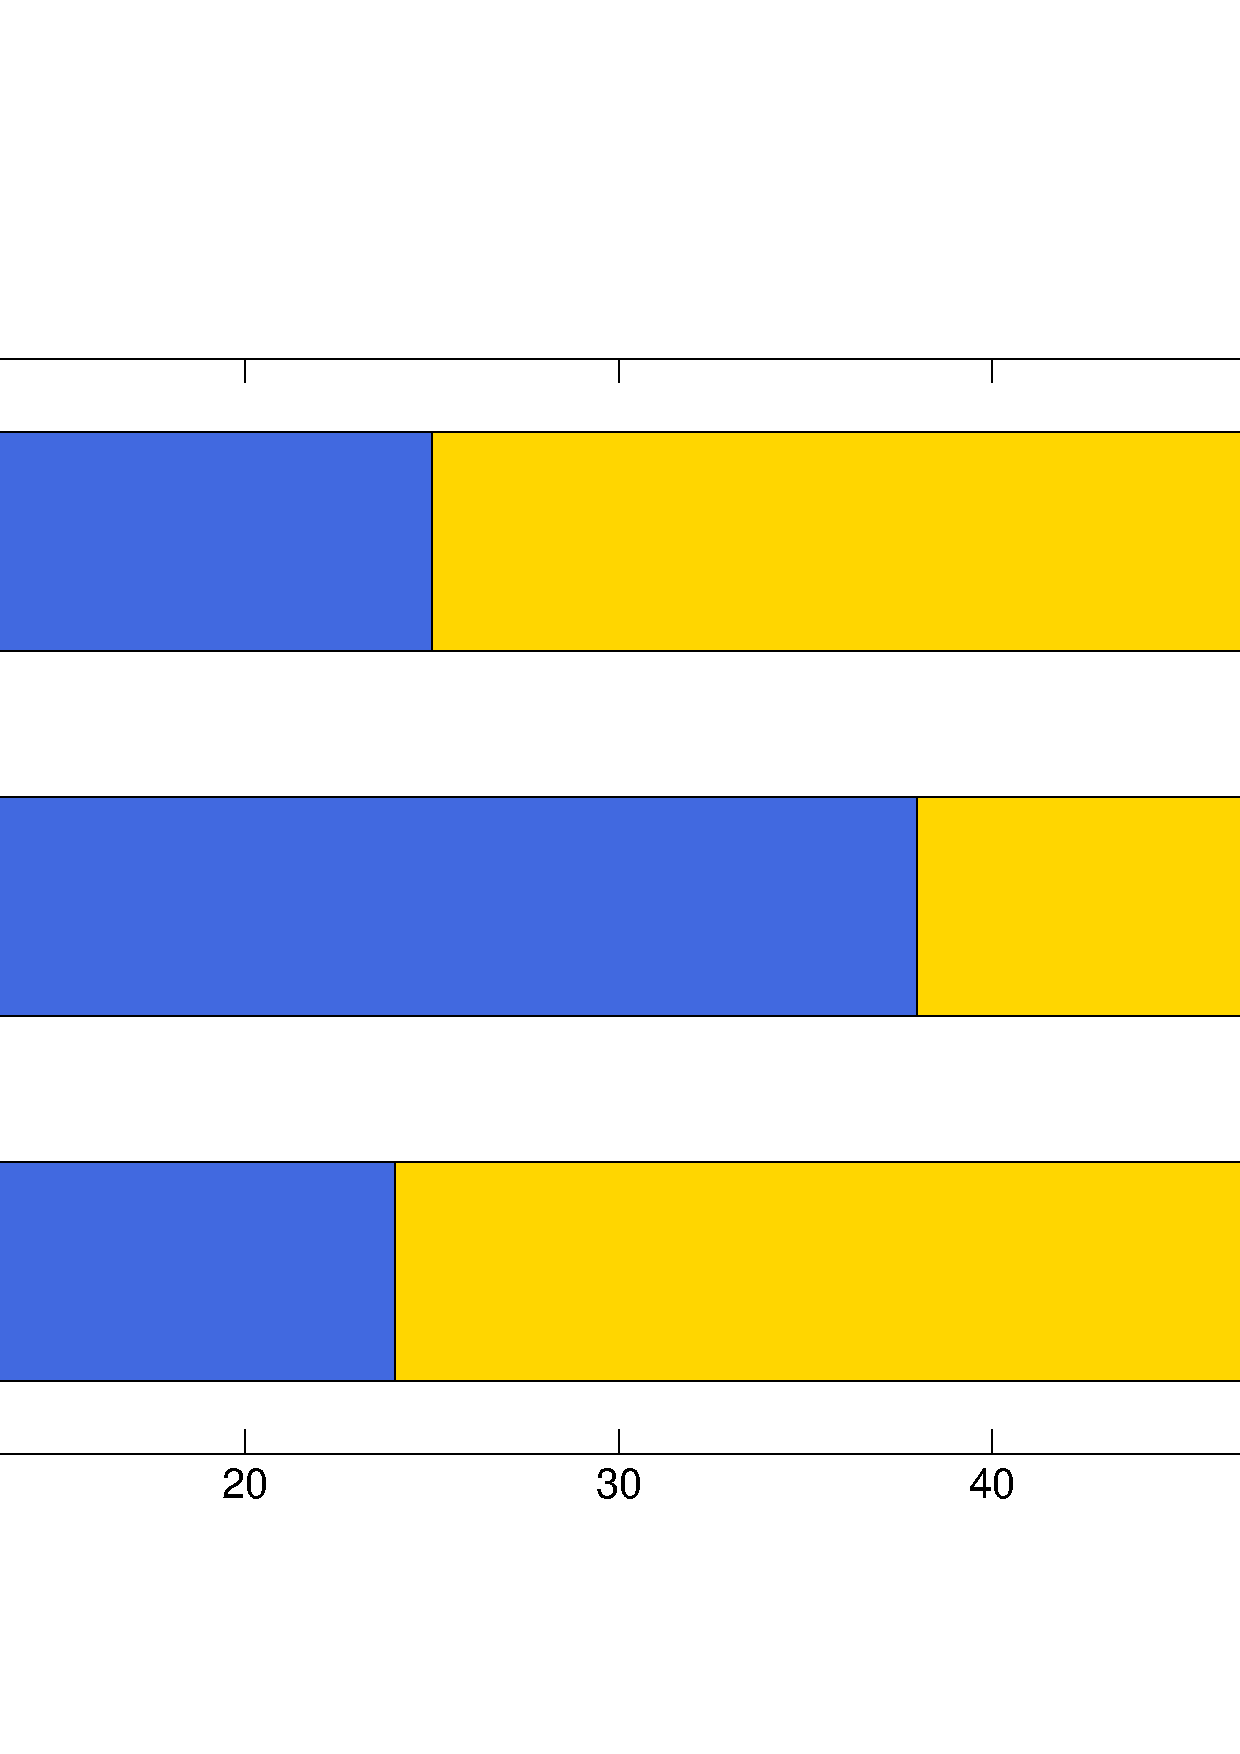
\includegraphics[width=\textwidth]{images/glott_vs_glott.pdf}
  \caption{Results of the AB test comparing different adapted voices obtained with the GlottHMM-based system}
  \label{fig:glott_vs_glott}
  \end{centering}
\end{figure}

In the first two cases, where the adapted voice using clean data and the clean configuration (both samples A) is compared to the one obtained using the noise reduction configuration and babble 20dB data, the results are pretty clear and show a preference to speech using clean data and a clean configuration ($p = 0.043$ and $p \ll 0.0001$).
%
For the third case, no significant conclusion can be formulated.

In Figure \ref{fig:glott_vs_st} the results of the AB test comparing GlottHMM-based system to the STRAIGHT-based are shown.
%
The comparisons made in these tests are all for the cases where babble noise is found on the background, as is the most common noise you could find when recording speech and also one of the hardest ones to deal with, due to its similar nature with speech.

These results show a slight preference for the GlottHMM samples over the STRAIGHT ones in the case of SNR 10dB and 20dB babble noise in the adaptation data.
%
The statistical significance test (binomial test) conducted shows that this preference is close to significant at best ( $p = 0.0516$ for SNR 20dB and $p \gg 0.05$ for SNR 10dB).
%
Nothing decisive can be said about the case where the adapted speech was obtained with the enhanced data.

\begin{figure}[!htb]
  \begin{centering}
  \includegraphics[width=\textwidth]{images/glott_vs_st.pdf}
  \caption{Results for the AB test comparing the performance of the GlottHMM-based system against the STRAIGHT-based one}
  \label{fig:glott_vs_st}
  \end{centering}
\end{figure}

Finally, Figure \ref{fig:mos_scores} presents the MOS scores for the listening test.
%
The STRAIGHT system is rated slightly higher in naturalness than the GlottHMM-based system for almost all the noise cases.
%
In similarity both systems are quite close, with STRAIGHT being slightly better in the case of babble at SNR 20dB.
%
Background quality is rated very evenly for the STRAIGHT-based systems, whereas the GlottHMM is highly affected when the SNR drops from 20dB to 10dB.

\begin{figure}[!htb]
  \begin{centering}
  \includegraphics[width=0.75\textwidth]{images/all_subjective_test_quality.pdf}
  \caption{Mean opinion scores (MOS) for the second part of the listening test. Median is denoted by the red line, boxes cover 25th and 75th percent percentiles, whiskers cover the data not considered outliers. The notches mark the 95\% confidence interval for the median}
  \label{fig:mos_scores}
  \end{centering}
\end{figure}
%\section{Introduction}

%% Leave first page empty
%\thispagestyle{empty}

%% In a thesis, every section starts a new page, hence \clearpage
%\clearpage



%% Three levels of hierarchy in sectioning should be enough

\clearpage

%% The \phantomsection command is nessesary for hyperref to jump to the 
%% correct page, in other words it puts a hyper marker on the page.

\phantomsection
%\addcontentsline{toc}{section}{Viitteet}
\addcontentsline{toc}{section}{References}
\bibliographystyle{ieeetr}
\bibliography{sections/references}



\appendix 
\clearpage
%% Adds the word "Appendices" to the table of contents
\addtocontents{toc}{\protect\contentsline{section}{Appendices}{}{appendix}}

 %% appendix example (starts with section) in Finnish
\section{GlottHMM Configuration}
\label{glott_conf}
%% Equations, tables and figures have their own numbering in Appendices, REMEMBER TO DO EVERY TIME YOU START AN APPENDIX, THE LETTER A IS THE APPENDIX INDEX
\renewcommand{\theequation}{A\arabic{equation}}
\setcounter{equation}{0}  
\renewcommand{\thefigure}{A\arabic{figure}}
\setcounter{figure}{0}
\renewcommand{\thetable}{A\arabic{table}}
\setcounter{table}{0}
\input{sections/glott_conf}

\newpage
\section{Questions of the Listening Test}
\label{test_questions}
\renewcommand{\theequation}{B\arabic{equation}}
\setcounter{equation}{0}  
\renewcommand{\thefigure}{B\arabic{figure}}
\setcounter{figure}{0}
\renewcommand{\thetable}{B\arabic{table}}
\setcounter{table}{0}

\begin{table}[!htb]
	\begin{framed}
	$\rhd$ \underline{Natural reference speech sample}\\
	$\rhd$ \underline{Synthesized speech sample A}\\
	$\rhd$ \underline{Synthesized speech sample B}\\
	\\
	Play the reference sentence. Then play both sample sentences. Considering the OVERALL QUALITY of the signal, select the one you would prefer to represent the reference voice in applications like mobile devices, video games, audio books etc. Regarding the OVERALL QUALITY
	\begin{itemize}
	\item[A.] First sample is better
	\item[B.] Second sample is better
	\item[C.] They sound exactly the same
	\end{itemize}
	\end{framed}
\caption{Questions used in the subjective evaluation AB test}
\label{table:abtest_questions}
\end{table}

\begin{table}[!htb]
	\begin{framed}
	$\rhd$ \underline{Synthesized speech sample}\\
	Play the sample and attending ONLY to the SPEECH SIGNAL, select the category which best describes the sample you just heard. The SPEECH SIGNAL in this signal was
	\begin{itemize}
	\item[5.] Completely natural
	\item[4.] Quite natural
	\item[3.] Somewhat unnatural but acceptable
	\item[2.] Quite unnatural
	\item[1.] Completely unnatural
	\end{itemize}
	\end{framed}
	\begin{framed}
	$\rhd$ \underline{Synthesized speech sample}\\
	Play the sample and attending ONLY to the BACKGROUND, select the category which best describes the sample you just heard. The BACKGROUND in this signal was
	\begin{itemize}
	\item[5.] Clean
	\item[4.] Quite clean
	\item[3.] Somewhat noisy but not intrusive
	\item[2.] Quite noisy and somewhat intrusive
	\item[1.] Very noisy and very intrusive
	\end{itemize}
	\end{framed}
	\begin{framed}
	$\rhd$ \underline{Natural reference speech sample}\\
	$\rhd$ \underline{Synthesized speech sample}\\
	Play both samples, and attending ONLY to the SPEECH SIGNAL, select the category which best describes the second sample to the reference sample.The voices in the SPEECH SIGNALS of the samples sounded
	\begin{itemize}
	\item[5.] Exactly like the same person
	\item[4.] Quite like the same person
	\item[3.] Somewhat different but recognizable
	\item[2.]Quite like a different person
	\item[1.] Like a totally different person
	\end{itemize}
	\end{framed}
	\caption{Questions used in the subjective evaluation MOS test}
\label{table:mostest_questions}
\end{table}
\end{document}
